\section{Timing Compartments}

This section introduces a new architecture abstraction, named timing 
compartments.
The goal of the timing compartment is to enable strong timing isolation
among multiple software components that share a multi-core processor,
similar to running each on a dedicated processor.
In that sense, the timing compartment provides hardware support that is 
necessary to remove 1) both side and covert timing channels, 2) among
different programs, 3) for a full processor.

%We first discuss the class of timing channels that timing compartments are 
%designed
%to prevent.  Then, we define the timing compartment, describe our threat model,
%and discuss application scenarios that timing compartments enable.

\subsection{Taxonomy of Timing Channels}

Timing channels exist whenever an adversary can correlate the timing of an event
to a secret data value. Adversaries exploit these vulnerabilities to extract 
secrets or undermine limitations on communication through timing rather than 
conventional means. In the context of this paper, we classify timing channels
into two types, {\em intra-program} and {\em inter-program}, 
based on the source of timing variations:

In an {\em intra-program} timing channel vulnerability, an adverasy can measure 
the time of a victim event directly and correlate this with a secret. For 
example, an adversary can attempt to authenticate to a remote site that uses a 
cryptographic protocol such as SSL and measure how long the server takes to 
respond. Bernstein's attack~\cite{bernstein} exploits an intra-program 
vulnerability in the AES implementation used in OpenSSL to extract the secret 
key. This vulnerability is caused by the program evicting its 
own cache misses or by repeated cold cache misses.
This and other {\em intra-program} timing channel vulnerabilities
exist even if a program runs on its own dedicated hardware.
Language-level techniques have been developed to
eliminate \cite{timesens} or mitigate \cite{mitigation1,mitigation2,mitigation3} 
such timing channels.

In contrast, {\em inter-program} timing channels are caused by interference 
between two programs that share hardware.
For example, Percival~\cite{percival} showed an {\em inter-program} timing 
channel attack where an adversarial program extracts another program's AES key
by measuring its own cache access time. The victim's (inadvertantly)
secret-dependent accesses interfere with the adverary's entries in the shared
cache allowing the adversary to correlate its own timings with the victim's key. 
Unlike intra-program timing chanels inter-program timing channels {\em can} be
eliminated if a program runs on a dedicated machine. Inter-program 
vulnerabilities are particularly troubling, because they can be exploited by an 
adversary that cannot measure victim events directly. For example, they can 
enable a malicious VM in a cloud infrastructure can steal secrets from a
co-resident VM that has no client-facing services.

Timing channel vulnerabilities can be exploited by side-channel or 
covert-channel attacks. In side-channel attacks, an adversary extracts a secret from
a victim program through unintentional timing variations.
In covert-channel attacks, two program collude to bypass restrictions and use
intentional timing variations to communicate.
While both attacks exploit timing variations, covert-channel protection requires
stronger control of timing variations. For example, inserting random noise may be
enough to prevent side-channel attacks, but typically cannot remove covert channels.

\subsection{Architecture Model}

%\subsection{Baseline Architecture}

    \begin{figure}
        \begin{center}
            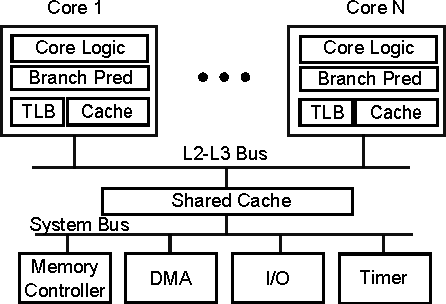
\includegraphics[width=3.04in]{figs/baseline.pdf}
            \caption{Baseline multi-core architecture.}
            \label{fig:baseline}
        \end{center}
    \end{figure}

Figure \ref{fig:baseline} shows a multi-core architecture that we assume
in this paper.
The architecture
has multiple cores, each with a core pipeline, a branch predictor, a TLB,
and one or more private caches (L1 and L2). 
The cores are connected to a shared cache (L3) via an on-chip bus. Then, a shared system 
bus connects the shared cache to a memory controller that manages requests to 
main memory as well as other system components such as a DMA engine, a timer, and I/O
modules.
For brevity, we do not consider simultaneous multithreading and assume that
cores cannot run multiple distrusting programs simultaneously.
However, a core may be time-shared (e.g. by context switching), and run multiple
programs over time.

%We assume that each core may be time shared by multiple timing
%compartments, but only one timing compartment, which we say is active, may run on each core
%at a time. This assumption can be relaxed if timing channel protection
%is added to per-core resources.

%\Ed{Perhaps move all the assumption that we make here?}

%Goal
%Timing compartments are designed to enable complete software isolation among
%entities that share hardware, comparable to having separate hardware for each.
%Assumptions
%Therefore, 
%we assume that a target system has multiple cores with shared
%resources such as caches, on-chip interconnects, and an off-chip memory that can
%be used by multiple programs concurrently. The system can also be time shared 
%(e.g. by context switching).
%The multicore system of interest consists of hardware resources that are
%concurrently shared by multiple software entities. It is possible for software 
%entities to be time multiplexed on the same core (e.g.  by context switching 
%VMs), but the system does not allow software entities to execute concurrently 
%on the same core (e.g. through simultaneous multithreading). 

\subsection{Security Model}

For security,
we assume that there exists a trusted software layer, such as an OS or a 
hypervisor, 
that handles conventional access control such as virtual memory and initializes 
and manages the timing compartments that address timing channels.
We refer to the OS/hypervisor module that manages timing compartments as
a timing compartment manager (TCM).
We address threats caused by one or more malicious programs running on a processor
which try to either extract information from another programs that run
concurrently, or communicate between them when no explicit communication is allowed. 

A timing compartment consists of  
software entities such as threads, processes, or virtual machines.
Our goal is to eliminate {\em inter-program} timing
channels among timing compartments which are caused through fine-grained sharing of microarchitecture 
resources\footnote{In general, this abstraction can be extended to support
more expressive policies based on the lattice model \cite{denning} to only prevent
a subset of timing channels.}.
To provide a level of isolation that is similar to running on a dedicated processor,
the timing compartment needs to prevent both side-channel and covert-channel attacks.
However, {\em intra-program} timing channels,
which exist even without shared hardware, are not prevented by
timing compartments. 

Timing compartments allow software to explicitly control timing channels
among groups of software entities, but does not enforce any restrictions within
each compartment. We believe that handling timing channels separately from
traditional isolation abstractions such as processes and virtual machines is 
essential to allow efficient system designs. Timing channel protection
is more expensive than traditional access control, so a designer should be able
to pay the overhead of timing channel control only when necessary.

In practice, multi-core systems have a number of shared sources even beyond a
processor chip, and comprehensive timing isolation cannot be achieved only in hardware.
Instead, we rely on trusted software such as an OS to prevent timing channels 
through events such as I/O or timer interrupts which are highly 
software-dependent.
These resources are directly managed by the OS/hypervisor and cannot be accessed 
without explicit system calls or hypercalls.
The role of a timing compartment is to eliminate
timing interference caused by fine-grained microarchitecture events such as memory accesses,
that cannot be controlled in software.
In our multi-core architecture model, timing compartments need to eliminate
timing interference in the shared memory hierarchy, including a shared cache,
on-chip interconnect, cache coherence mechanisms, and a memory controller.

%Timing 
%channels between timing compartments are allowed or prevented based on a policy 
%specified in software.  Policies are specified by a lattice of security levels
%where leakage is prevented from preceeding levels to preceded levels.
%of a lattice model, which defines ordering between security levels 
%\cite{denning}.
%This lattice model is quite expressive and widely used for information flow 
%control. 

In the current implementation of the protection mechanisms, we also assume that
timing compartments have separate address spaces and do not share physical
pages except for read-only pages that are commonly used for program code.
There is no point in timing isolation if explicit communication is allowed.
%Communications between timing compartments are controlled through the 
%trusted
%software layer and be explicitly managed to prevent external timing channels. 

%Attacks we handle.
%However, these approaches to isolate software do not address timing channels 
%that leverage shared hardware. To guarantee total isolation, internal timing 
%channels must also be eliminated. We eliminate all internal microarchitectural 
%timing channels including state and state-based timing channels.  This includes 
%all timing channels caused by concurrently shared resources as well as timing 
%channels in hardware that is shared through time multiplexing (e.g.  by context 
%switching).

%Timing compartments aim to eliminate {\em internal} timing channels through
%interference in shared microarchitecture resources. In particular, the goal is
%to prevent both unintentional (side channel) and intentional (covert channel)
%information leaks.
%However, external timing
%channels, which exist even without shared hardware, are not prevented by
%timing compartments. If necessary, the external timing channels can be 
%controlled in software. Similarly, timing channels through I/O devices are not 
%considered in this study,
%because they may be prevented in software.
%Finally, we do not consider attacks that require physical access such as
%side-channel attacks through power consumption or electromagnetic emission.

%Attacks we don't handle.
%Since our goal is to address vulnerabilities caused by hardware sharing,
%timing channels that are external to the hardware are not addressed.
%Any timing channels that are external to the hardware in this system would also 
%be present if the software entities executed on separate hardware. If 
%necessary, external timing channels can be controlled in software. Similarly, 
%we do not address language level timing channels since these may also be 
%addressed in software.  Lastly, we do not consider physical attacks and assume 
%that the adversary does not have physical access.


%\Ed{We need to talk about what we need to cover in the timing compartment. 
%We assume that software can handle timing channels through resources that
%are accessed through an OS. So the timing compartment will only cover the
%hardware resources that are concurrently shared w/o explicit control?}


%\subsection{Definition of Timing Compartments}

%Timing compartments are a new architecture abstraction that allows software to
%explicitly control {\em internal timing channels} in shared systems.
%When used in conjunction with access
%control mechanisms, such as conventional page handlers, they provide complete software 
%isolation, because timing channels are the only side/covert channels that can be
%exploited in software without physical attacks.

%As a software level abstraction, a timing compartment consists of one or more 
%software entities such as threads, processes, and virtual machines.  Timing 
%channels between timing compartments are allowed or prevented based on a policy 
%specified in software.  Policies are specified by a lattice of security levels
%%where leakage is prevented from preceeding levels to preceded levels.
%%of a lattice model, which defines ordering between security levels 
%\cite{denning}.
%This lattice model is quite expressive and widely used for information flow 
%control. 

%  For example, the lattice may restrict timing channels only in one direction 
%  from $\mathtt{TC1}$ to $\mathtt{TC2}$ ($\mathtt{TC2} \leq \mathtt{TC1}$).
%  The lattice may disallow any timing channel between two compartments by 
%  making
%  them incomparable ($\mathtt{TC_1} \nleq \mathtt{TC_2}$, $\mathtt{TC_2} \nleq 
%  \mathtt{TC_1}$).

%Here, a software entitiy is some system abstraction (such as processes or 
%threads in a single OS system or virtual machines in a virtualization based 
%system) that execute software and have an owner. Intuitively, a single timing 
%compartment contains only software entities that trust each other explicitly 
%(such as all the VMs on a machine owned by the same user) or implicitly (all 
%the VMs that do not want to pay for protection), and leakage within a timing 
%compartment is safe.

%Similar to other architecture abstractions such as virtual memory,
%timing compartments are implemented as a combination of hardware and software
%mechanisms. The underlying hardware must provide mechanisms to distinguish
%events from different timing compartments and control timing interference in 
%shared resources. Then, a trusted software component, which we call the timing 
%compartment manager (TCM) manages the hardware mechanisms at run-time.

%To enforce the policy, a trusted software component called the timing 
%compartment manager (TCM) confines software entities into TCs. The TCM then 
%informs the hardware of the TCs and policy. At runtime, the TCM tags software 
%requests for hardware to indicate the TC of the software entity that made the 
%request. The hardware then enforces the policy by controlling how requests from 
%different TCs share resources.

%Timing compartments only address timing channels; they do not control 
%information flow through explicit channels. Handling these concerns separately 
%allows for more flexibility in the overall system design.  When designing a 
%secure system, implementors must consider how the cost required to carry out a 
%particular attack compares with other attacks, the potential damage that could 
%be caused by an attack, and the cost and performance impact of implementing the 
%security mechanisms needed to stop it. This enables timing compartments to 
%provide timing channel protection only to software entities that need it.

\subsection{Application Scenarios}

The ability to control inter-program timing channels can significantly increase the
level of
assurance in diverse application domains where distrusting entities share a
physical system. Here, we briefly discuss representative applications.

\subsubsection{Bring Your Own Device (BYOD)}

Now that mobile devices such as smartphones and tablets are widely used, 
companies and government organizations are starting to allow employees to
use their own devices to access the organization's data.
Bring Your Own Device (BYOD) platforms intend to enable this. However, there is 
concern that mixed use can lead to a leak of confidential data through personal 
emails or
downloaded applications. BYOD solutions such as Samsung Knox use
software containers or virtualization to separate the two environments:
personal and work. Yet, these solutions cannot prevent information leaks
through timing channels.

\begin{figure}
    \begin{center}
        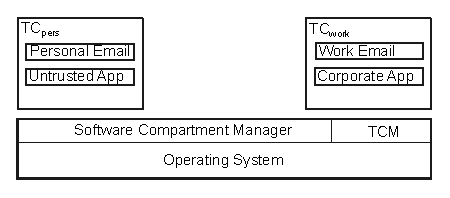
\includegraphics{figs/byod.eps}
        \caption{A BYOD example.}
        \label{fig:byod}
    \end{center}
\end{figure}

Timing compartments enable stronger isolation guarantees for BYOD
platforms. For example, consider the solution based on virtualization shown in 
Figure~\ref{fig:byod}. The virtual machines for
work and personal use are assigned to two different timing compartments:
$TC_{work}$ and $TC_{pers}$. 
%The policy is configured so that no information can 
%flow from $TC_{work}$ to $TC_{pers}$.
Note that the BYOD application only requires two timing compartments even
though a system may have many cores and run many applications.

\subsubsection{High-Assurance Cloud Computing}

Infrastructure as a service cloud providers, such as Amazon EC2, lease virtual 
machines (VMs) that share physical hardware. 
%A cloud provider co-locates many VMs on a single machine to increase its 
%utilization,
%and tenants often have little control over where their VMs run.
A tenant may share hardware with competitors or attackers that want
to extract sensitive data. Conventional virtualization technologies restrict 
explicit
communication channels among virtual machines, but cannot control 
timing channels. A practical timing channel attack has been exploited
in commercial clouds to extract cryptographic keys\cite{heyyou}.
For some clients, timing channels may not be a concern. Yet, for enterprise or 
government clients who require high assurance,
this security threat makes public cloud computing unusable. 

\begin{figure}
    \begin{center}
        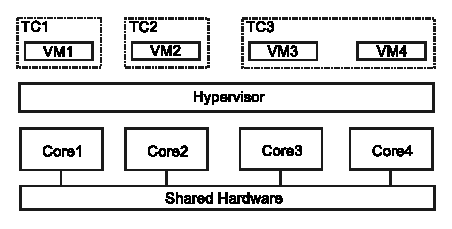
\includegraphics{figs/cloud_tcs.eps}
        \caption{A cloud computing example. VM1 and VM2 have high security 
        requirements, but VM3 and VM4 do not.}
        \label{fig:cloud_tcs}
    \end{center}
\end{figure}

Timing compartments can enable high assurance cloud computing by preventing
unintended information leakage among virtual machines.
Figure~\ref{fig:cloud_tcs} shows a cloud computing environment with four virtual 
machines (VMs).
%that have different security requirements. 
VM1 and VM2 require a strong isolation guarantee and distrust each other and 
other VMs.
VM3 and VM4 run low-security applications that do not require timing channel 
protection, but require high performance. The figure shows how three timing 
compartments can be used to meet the security requirements in this example.
VM1 and VM2 are placed in their own timing compartments $TC1$ and $TC2$, but VM3 
and VM4 are grouped in $TC3$. 
%The policy prevents leakage out of $TC1$ and 
%$TC2$, but places no constraint on timing channels out of $TC3$. 
This meets the 
security requirements of VM1 and VM2, but VM3 and VM4 are allowed to share 
resources normally for improved performance.


\subsubsection{Untrusted Software} 

The ability to completely eliminate timing channels enables timing compartments
to be used to contain information even when software is potentially malicious.
For example, smartphone users download third party applications
that cannot be fully trusted to manage private or sensitive data. A system may
sandbox an untrusted application and restrict its communication channels
when it accesses sensitive data. However, access control mechanisms cannot
prevent the untrusted application from leaking information to another 
unrestricted
application through covert timing channels. The timing compartment can 
be added to provide a complete sandbox.  In a cloud computing
context, the same timing channel protection can be used
by a cloud provider to sandbox third-party web services that cannot be fully 
trusted.

\subsubsection{Safety-Critical Systems}

In addition to protecting confidential data, the capability to control 
interference in shared hardware can also be used to provide timing guarantees on 
safety-critical systems. For example, hard real-time systems such as automotive 
controllers must meet strict timing requirements. Unfortunately, multi-core
processors cause interference that makes timing guarantees impossible. Timing
compartments can be used to ensure that the timing of safety-critical components 
are not affected by the rest of a system.

